
%(BEGIN_QUESTION)
% Copyright 2007, Tony R. Kuphaldt, released under the Creative Commons Attribution License (v 1.0)
% This means you may do almost anything with this work of mine, so long as you give me proper credit

Explain how this motor control circuit (sometimes referred to as a ``bucket'') works for an electrically-actuated gate valve:

$$\includegraphics[width=15.5cm]{i01824x01.eps}$$

Explain the function and purpose of each switch in the ladder logic circuit.

\underbar{file i01824}
%(END_QUESTION)





%(BEGIN_ANSWER)

When closing a gate valve, you want the gate to wedge firmly against the valve seat for tight shutoff.  However, it does not matter as much whether or not the gate is fully withdrawn when the valve is wide open.
 
%(END_ANSWER)





%(BEGIN_NOTES)

%INDEX% Final Control Elements, valve: electric actuator

%(END_NOTES)


